\documentclass[12pt]{article}

\title{Application of Machine Learning Coursework Report}
\author{James Hughes}

\bibliographystyle{unsrt}

\usepackage{graphicx}
\usepackage{subcaption}

\begin{document}

\maketitle

\newpage

\tableofcontents

\newpage

\section{Gaussian Noise Diffusion}
\subsection{Diffusion Model \& Training Algorithm}
The code found in the repository for this project was based on the Jupyter notebook found in the \texttt{assignment} directory.
This notebook contains a standard pipeline which trains a Denoising Diffusion Probabilistic Model,
a kind of generative model first appearing in the literature just four years ago \cite{ho2020denoising}.
The model is trained using the training partition of the MNIST dataset \cite{mnist}, which contains monochrome images of handwritten digits.

Fundamental to this model is an underlying image-to-image convolutional neural network,
which tries to predict a ground truth MNIST image from the same image, with added Gaussian noise, as an input.
This netowrk has a deep, symmetrical architecture based on convolutional layers which initially increase the number of channels,
which extracts features from the input, and then later combines these channels to eventually produce a monochrome (single-channel) generated image.
These convolutional layers are combined with a layer normalisation,
which normalises the pre-activations of the hidden units separately for each input of the batch \cite{ba2016layer}.
This step builds on the batch normalisation approach, improving the stability and speed of training the neural network \cite{ba2016layer},
but has the advantage of being more suitable when batches are small or have a large within-batch variation \cite{prince2023understanding}.
The results of the layer normalisation are then passed through a GeLU activation function \cite{hendrycks2023gaussian},
which is a close variant of the standard ReLU activation function,
but which mitigates the issue of vanshing gradients by having non-zero gradients for small negative inputs \cite{nguyen2021analysis}.

The underlying CNN model also takes a scalar time step \texttt{t} in $[0,1]$ as part of its raw input; this becomes a vector when inputs are batched,
with one scalar for each batch member.
Each of these scalars is in turn encoded as a vector, whose entries are a periodic function (of progressively increasing frequency)
of the scalar value.
These vectors are then passed through a series of learned linear layers and non-linear activations,
changing their length to equal the number of hidden channels in the first layer of the CNN.
These time embeddings are then combiend with the first hidden activations via addition.

This underlying model is then wrapped in a \texttt{DDPM} class, implementing a \texttt{forward} and \texttt{sample} method.
The \texttt{forward} method takes a batch of MNIST images input.
It generates a random time step for each image, which controls the strength of degradation applied to each,
taking the form of addition with Gaussian pixel noise.
It feeds the degraded image and the time step to the CNN, and returns the mean squared error between the CNN output and the original noise map.
During training this incentivises the CNN to predict the Gaussian noise applied to a degraded image.
The \texttt{sample} method implements Algorithm 18.2 in \cite{prince2023understanding}.
It starts with a random Gaussian tensor the same size as the MNIST images, which it then passes through the trained CNN,
and subsequently degrades with Gaussian noise.
These two transformations are repeated for smaller and smaller timesteps until the degradation is minimal.

The initial codebase was created by refactoring this notebook into a library, \texttt{diffusiontools}.
The training procedure was then altered to make training runs more repeatable.
Alongside the samples which were produced at each epoch, the trained model was itself saved as a \texttt{.pt} file.
This enabled further investigation into intermediate models after the training, and indeed meant that later on,
the periodic sampling could be removed altogether to speed up training (as sampling could be done in post).
The hyperparameter settings were also controlled via a \texttt{config.ini} to enable different configurations to be easily tested, and tracked.

\subsection{Analysis of Training}

\begin{figure}[hp]
    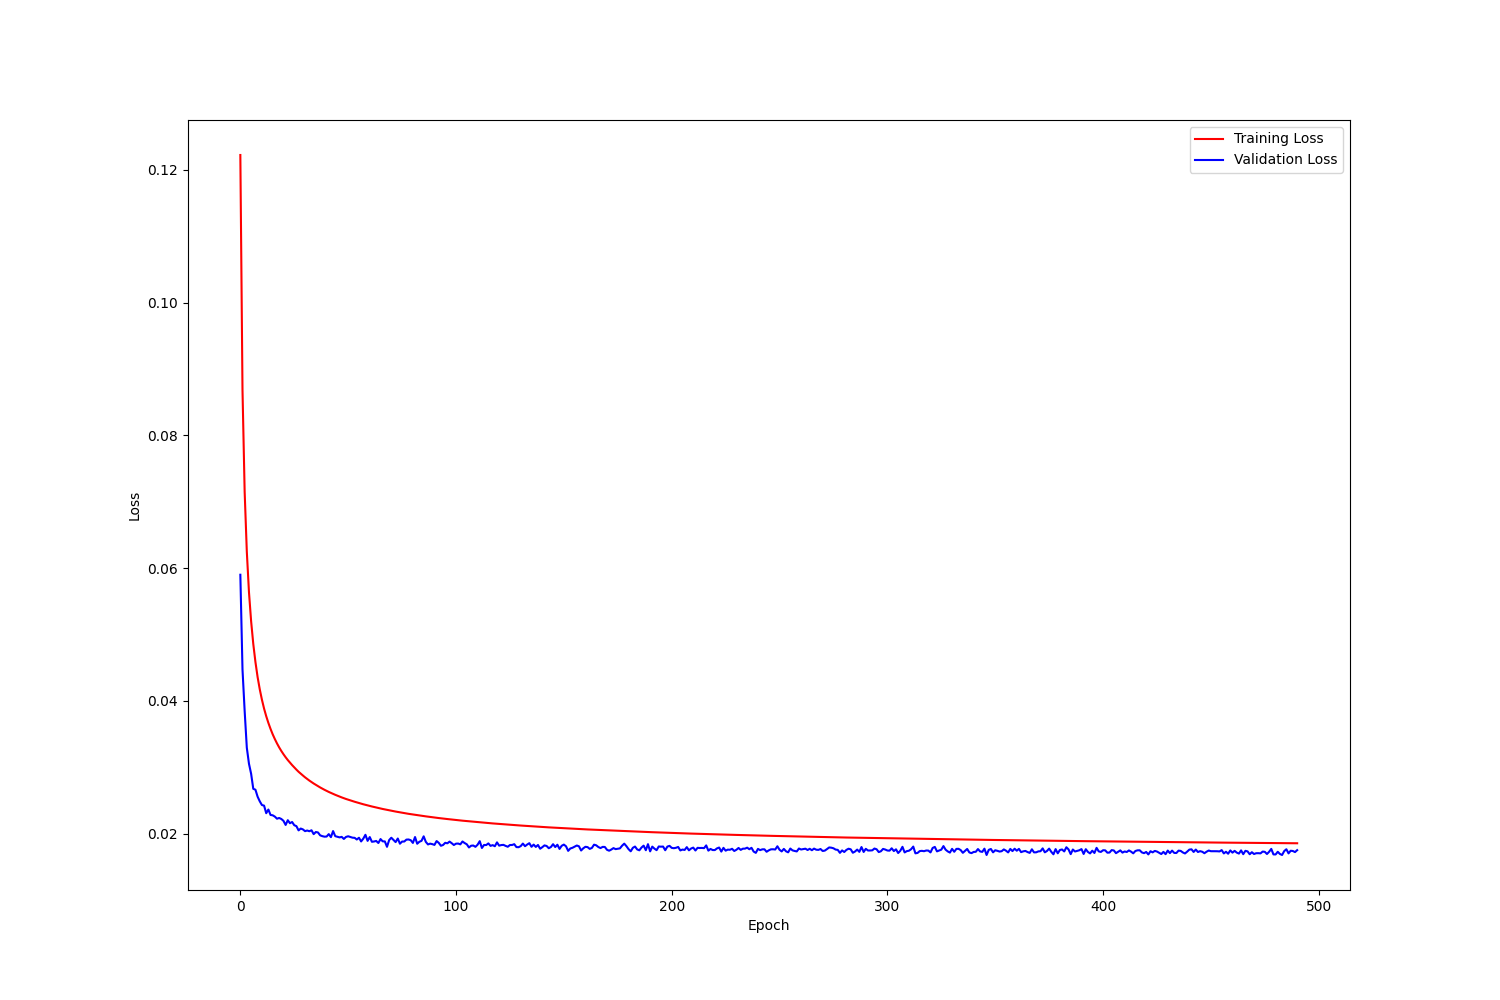
\includegraphics[scale=0.35]{figures/learning_curve_1.png}
    \caption{Learning Curve for Model 1 Trained over 500 Epochs.}
    \label{fig:learning_curve_1}
\end{figure}

The first model trained had the same hyperparameters as found in the notebook.
It was trained for 500 epochs by uploading the repository to the CSD3 systems.
The MNIST training dataset was split further into a training set (80\%) and a validation set (20\%),
to monitor the model's ability to generalise during the training process.

In Figure \ref{fig:learning_curve_1}, it can be seen that the validation loss appears to converge roughly around the 100 epoch stage,
with no significant improvements from further training.
This matches the findings of generated samples in Figure \ref{fig:diffusion_1}.
We see that around the 40 epoch mark, the model begins to produce symbols but these are not recognisable digits.
The images generated at epoch 60 are the first that resemble numerical digits --
images in Figure \ref{fig:diffusion_1}\ref{sub@fig:1_60} appear to show a 7, 5, 2, 1, and 9.
Figure \ref{fig:diffusion_1}\ref{sub@fig:1_120} appears to show higher fidelity images in the first three samples,
although the other two cannot be discerned as digits.
This model was selected for further analysis as the final trained model.

\begin{figure}[hp]
    \begin{subfigure}{0.49\textwidth}
    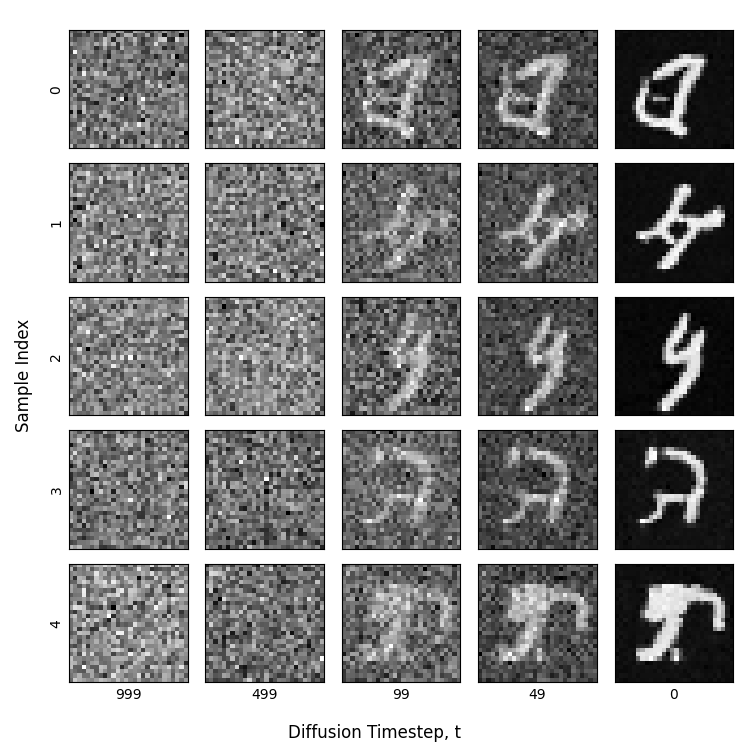
\includegraphics[width=0.9\linewidth, height=6cm]{figures/diffusion_plot_1_0040.png}
    \caption{Epoch 40}
    \label{fig:1_40}
    \end{subfigure}
    \begin{subfigure}{0.49\textwidth}
    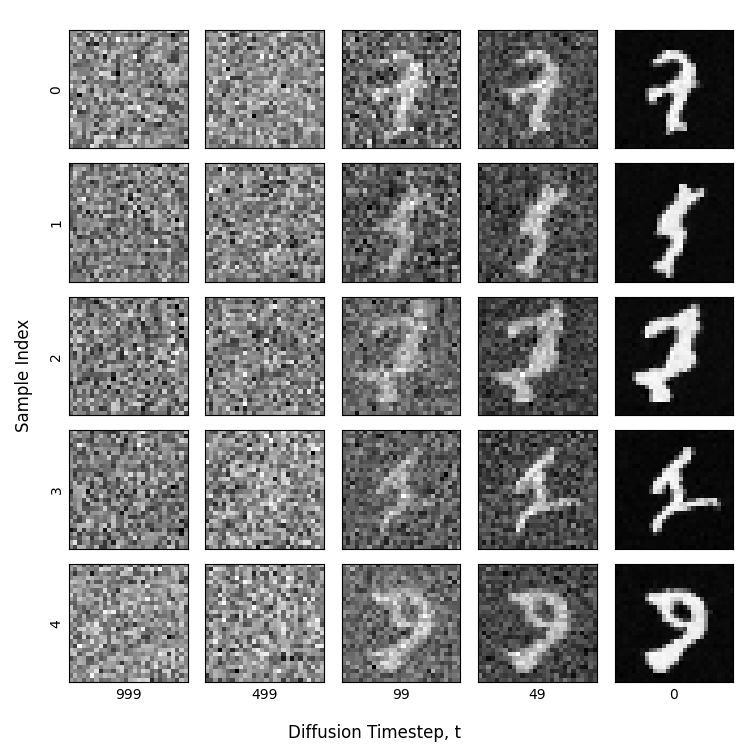
\includegraphics[width=0.9\linewidth, height=6cm]{figures/diffusion_plot_1_0060.png}
    \caption{Epoch 60}
    \label{fig:1_60}
    \end{subfigure}

    \begin{subfigure}{0.49\textwidth}
    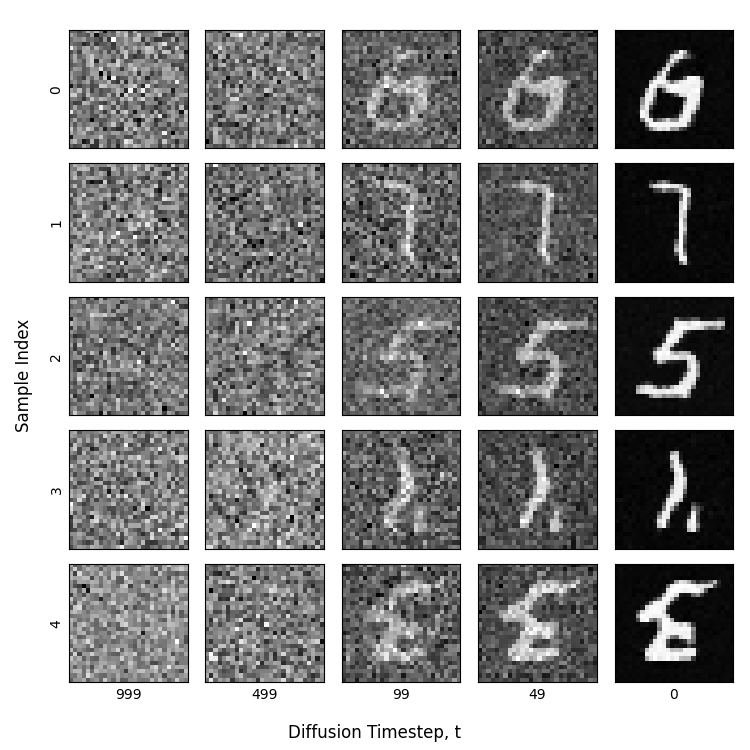
\includegraphics[width=0.9\linewidth, height=6cm]{figures/diffusion_plot_1_0120.png}
    \caption{Epoch 120}
    \label{fig:1_120}
    \end{subfigure}
    \begin{subfigure}{0.49\textwidth}
    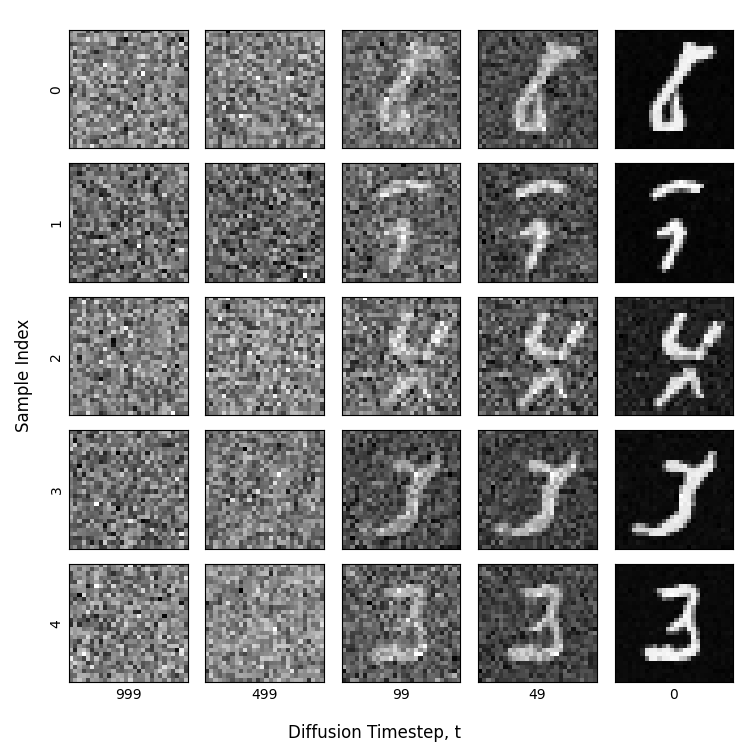
\includegraphics[width=0.9\linewidth, height=6cm]{figures/diffusion_plot_1_0300.png}
    \caption{Epoch 300}
    \label{fig:1_300}
    \end{subfigure}

    \caption{Model 1 diffusion process samples at various stages of training.}
    \label{fig:diffusion_1}
\end{figure}

A second similar model was then trained with a slightly different Gaussian noising schedule.
In this second model, the number of discrete timesteps in the diffusion process was reduced ten-fold to 100.
The noise parameter limits were accordingly increased by a factor of ten, ensuring that the amount of signal-to-noise ratio of an image at the final time step remained approximately zero.


\begin{figure}[hp]
    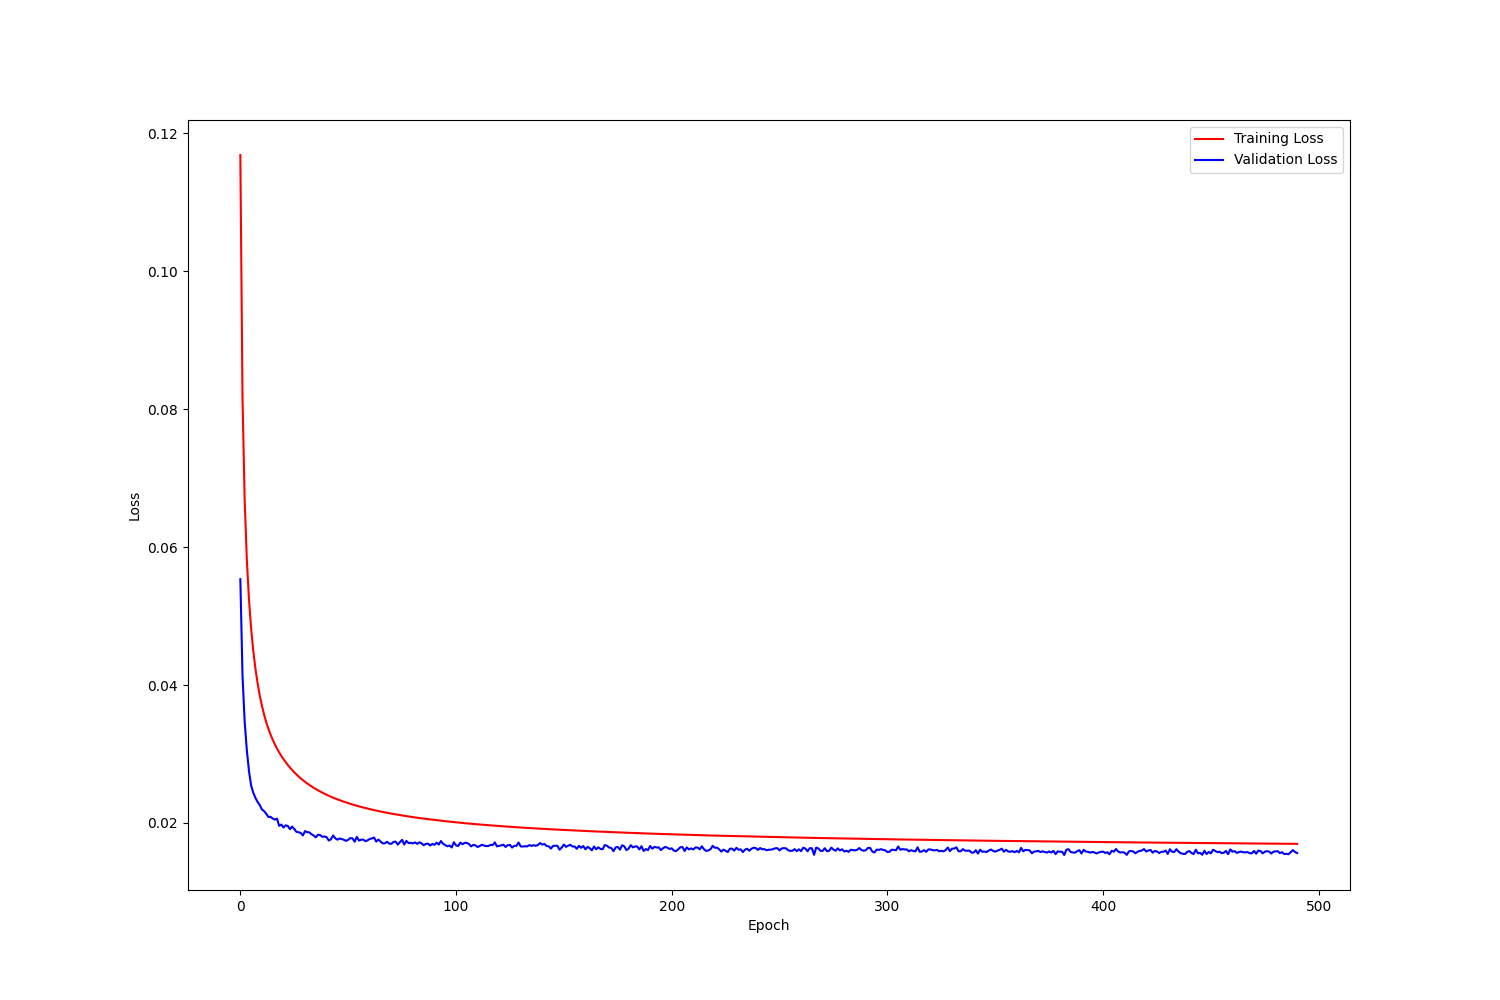
\includegraphics[scale=0.35]{figures/learning_curve_2.png}
    \caption{Learning Curve for Model 2 Trained over 500 Epochs.}
    \label{fig:learning_curve_2}
\end{figure}

\begin{figure}[hp]
    \begin{subfigure}{0.49\textwidth}
    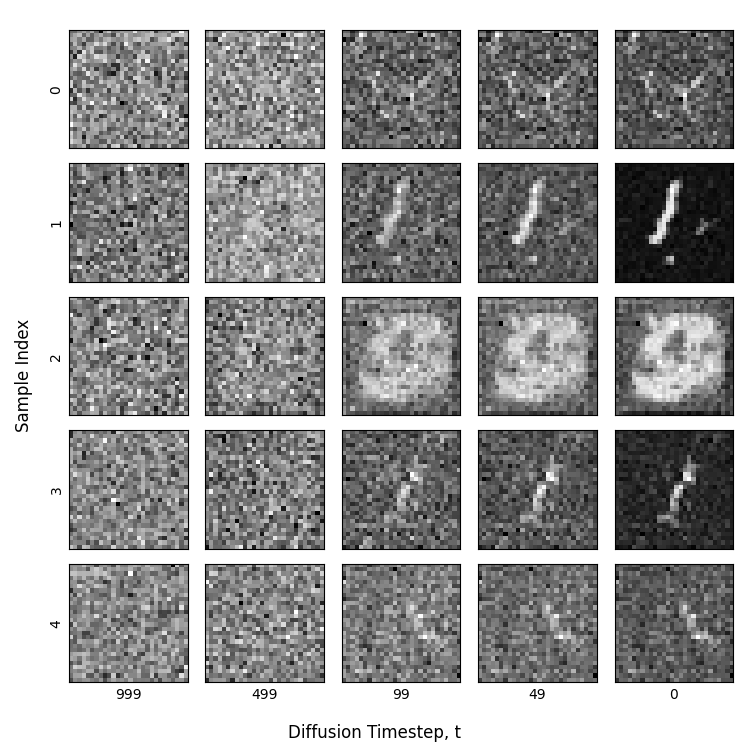
\includegraphics[width=0.9\linewidth, height=6cm]{figures/diffusion_plot_2_0020.png}
    \caption{Epoch 20}
    \label{fig:2_20}
    \end{subfigure}
    \begin{subfigure}{0.49\textwidth}
    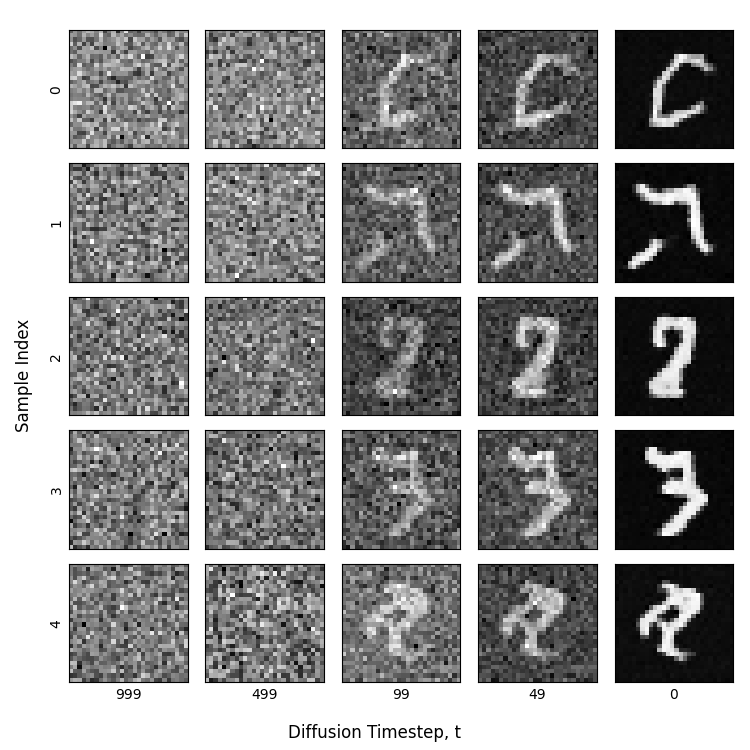
\includegraphics[width=0.9\linewidth, height=6cm]{figures/diffusion_plot_2_0040.png}
    \caption{Epoch 40}
    \label{fig:2_40}
    \end{subfigure}

    \begin{subfigure}{0.49\textwidth}
    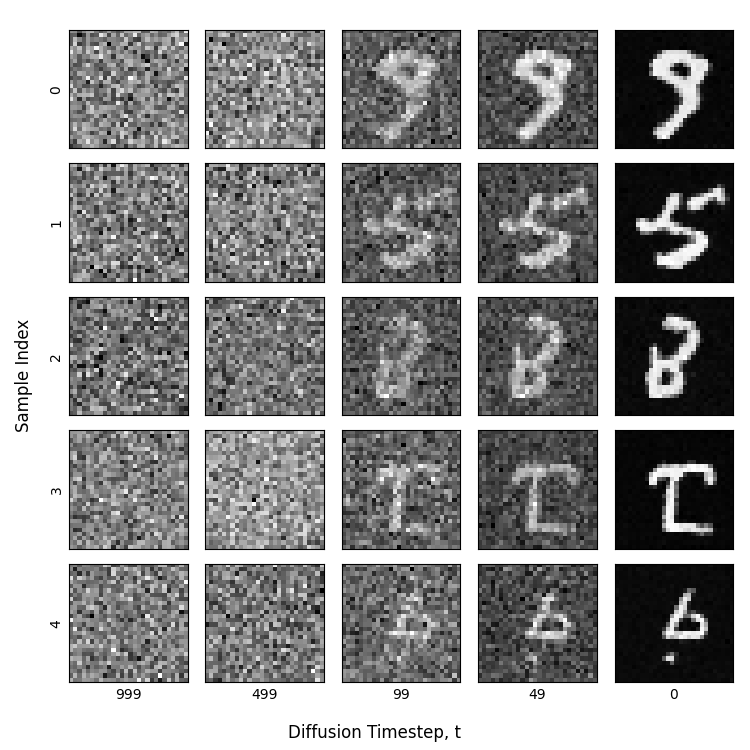
\includegraphics[width=0.9\linewidth, height=6cm]{figures/diffusion_plot_2_0080.png}
    \caption{Epoch 80}
    \label{fig:2_80}
    \end{subfigure}
    \begin{subfigure}{0.49\textwidth}
    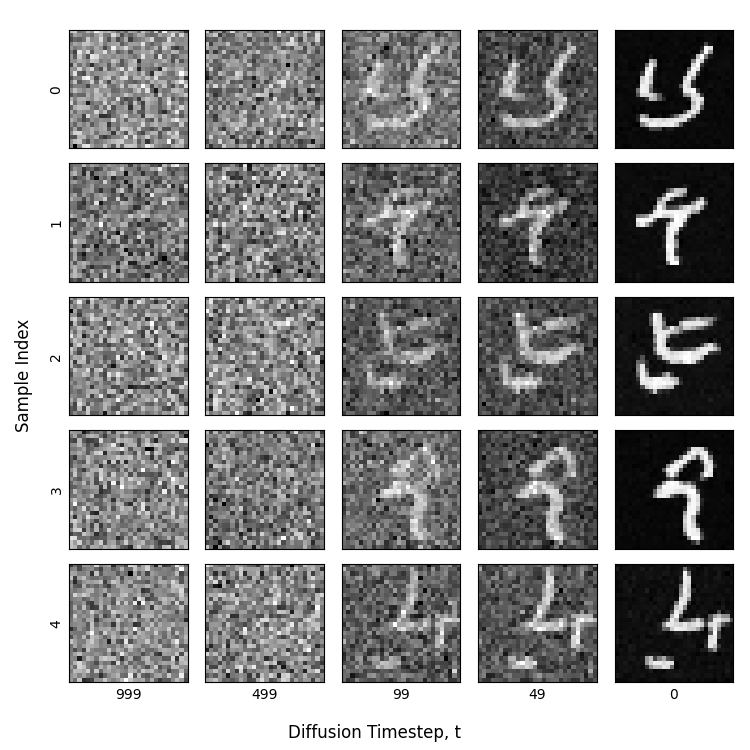
\includegraphics[width=0.9\linewidth, height=6cm]{figures/diffusion_plot_2_0100.png}
    \caption{Epoch 100}
    \label{fig:2_100}
    \end{subfigure}

    \caption{Model 2 diffusion process samples at various stages of training.}
    \label{fig:diffusion_2}
\end{figure}

A similar learning curve can be seen for the training of the second model in Figure \ref{fig:learning_curve_2}.
However, inspecting some of the images produced by intermediate models shows that the quality of the generated images deteriorates much earlier than in Model 1.
Even images produced at epoch 100 in \ref{fig:diffusion_2} appear to be low quality, with `fragmented' symbols rather than one continuous digit.
The images produced at epoch 80 appear to be the highest quality and this model was used in the final analysis.

\subsection{Analysis of Final Models}
The evaluation of generative models is a challenging and ongoing subject of research \cite{betzalel2022study},\cite{fi15080260}.
Unlike other tasks within machine learning such as classification, regression, and clustering,
an ideal generative model generalises from its training data to produce content that is simultaneously novel, diverse and realistic.
When diffusion models are used in a conditional generation setting, ground truth images can be degraded and then reconstructed by the diffusion model,
allowing evaluation through image comparison metrics such as SSIM and MSE, as done in \cite{bansal2022cold} -- this is explored later.
More broadly, a standard evaluation metric is the Fr\'echet Inception Distance \cite{NIPS2017_8a1d6947}.
In this project, the models are quantitatively assessed with the framework of comparing the statistical distributions of generated and ground truth images,
just like with the FID score, but in a slightly simpler and more interpretable way.
200 samples were taken from each of the four final models and combined with the 10,000 MNIST test images into a single array.
These were then transformed into two dimensions using t-SNE dimensionality reduction.
The effect of this on the MNIST dataset alone can be seen in Figure \ref{fig:tsne_mnist},
which shows that this technique is strikingly effective at encoding the true image class in a meaningful way.
A Gaussian mixture model with 10 components (corresponding to the 10 digits) was then fitted to each sample,
enabling an estimate of the KL divergence between the generated and ground truth image distributions.



\begin{figure}[hp]
    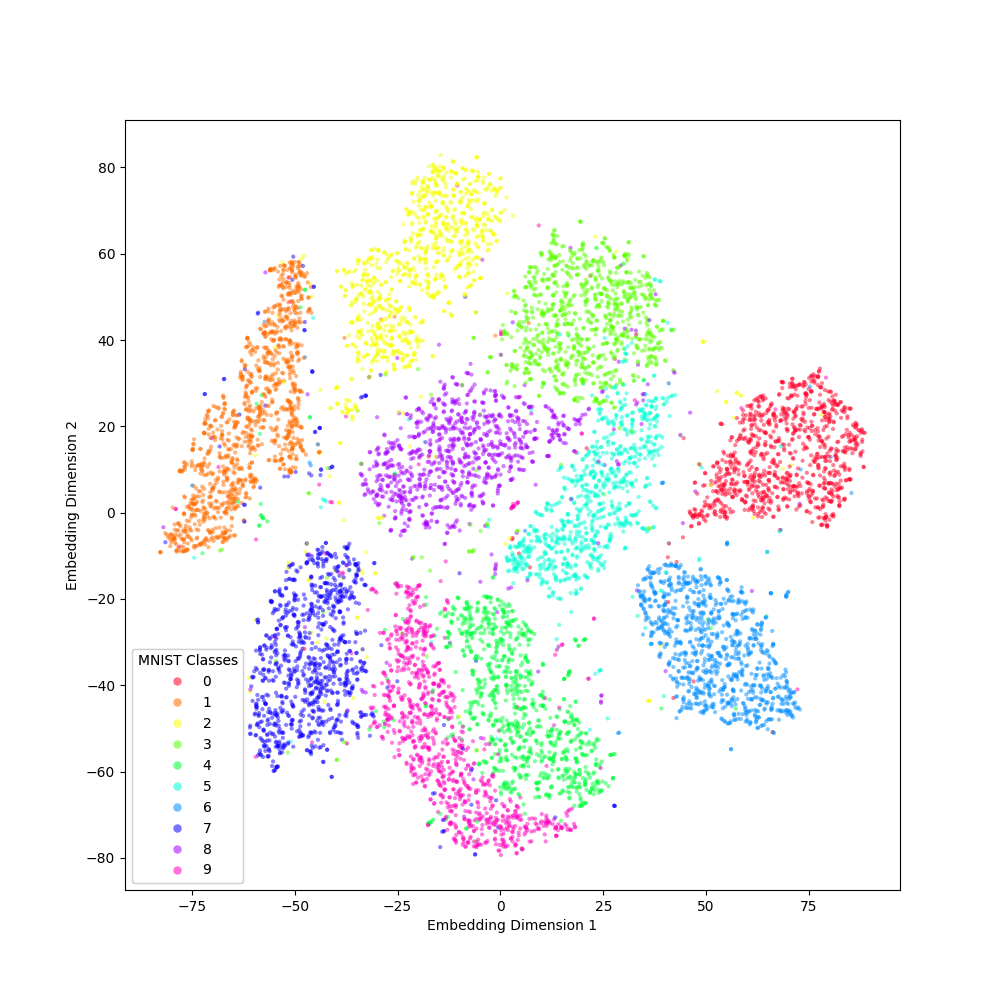
\includegraphics[scale=0.54]{figures/tsne_mnist.png}
    \caption{t-SNE dimensionality reduction applied to MNIST test dataset, with ground truth labels indicated.}
    \label{fig:tsne_mnist}
\end{figure}

\begin{figure}[hp]
    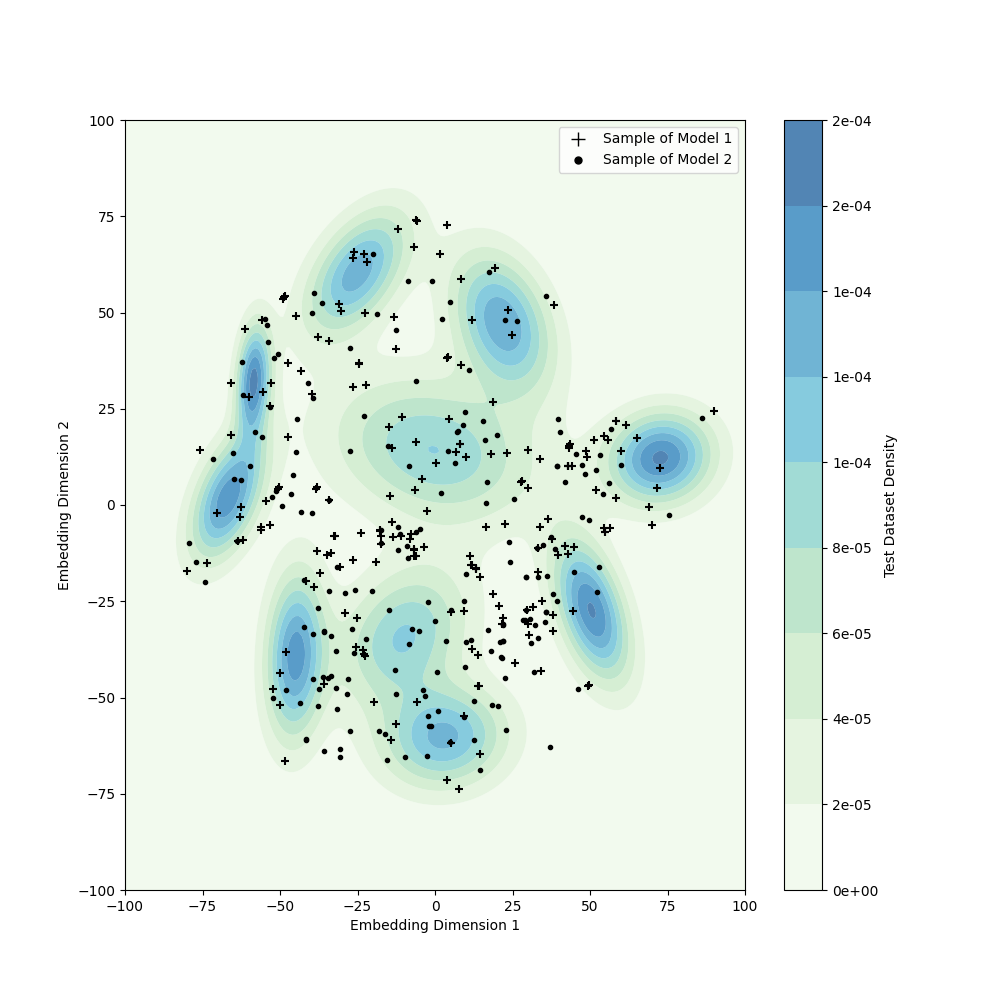
\includegraphics[scale=0.54]{figures/tsne_gaussian_models.png}
    \caption{t-SNE dimensionality reduction applied to Gaussian model samples, with contour plot of GMM density estimate for MNIST test data.}
    \label{fig:tsne_gaussian}
\end{figure}

Figure \ref{fig:tsne_gaussian} shows that both models have good coverage across the whole distribution of ground truth distribution of data,
suggesting they are capable of producing a variety of different digits.
However, we can also observe that neither distribution of points appears to have a similar clustering pattern to the ground truth data,
which suggests that both models also have a tendency to produce low quality samples that do correspond to a discernible digit.
The KL divergences, computed as $D_KL(P||Q)$ where $Q$ is the ground truth distribution, were similar with the model 1 sample at 0.81844,
and the model 2 sample at 0.77298.
This suggests that the distributions of generated images from both models imitate the ground truth with similar success.
When their images are treated as random vectors, the total variance (trace of the covariance matrix) for the first sample was 56.7,
and slightly higher for the second at 69.9.
While this may suggest a greater diversity of samples from the second model, it may also reflect the greater noise present at each step,
which in turn is clearly visible as the samples produced appear grainier.

\begin{figure}[hp]
    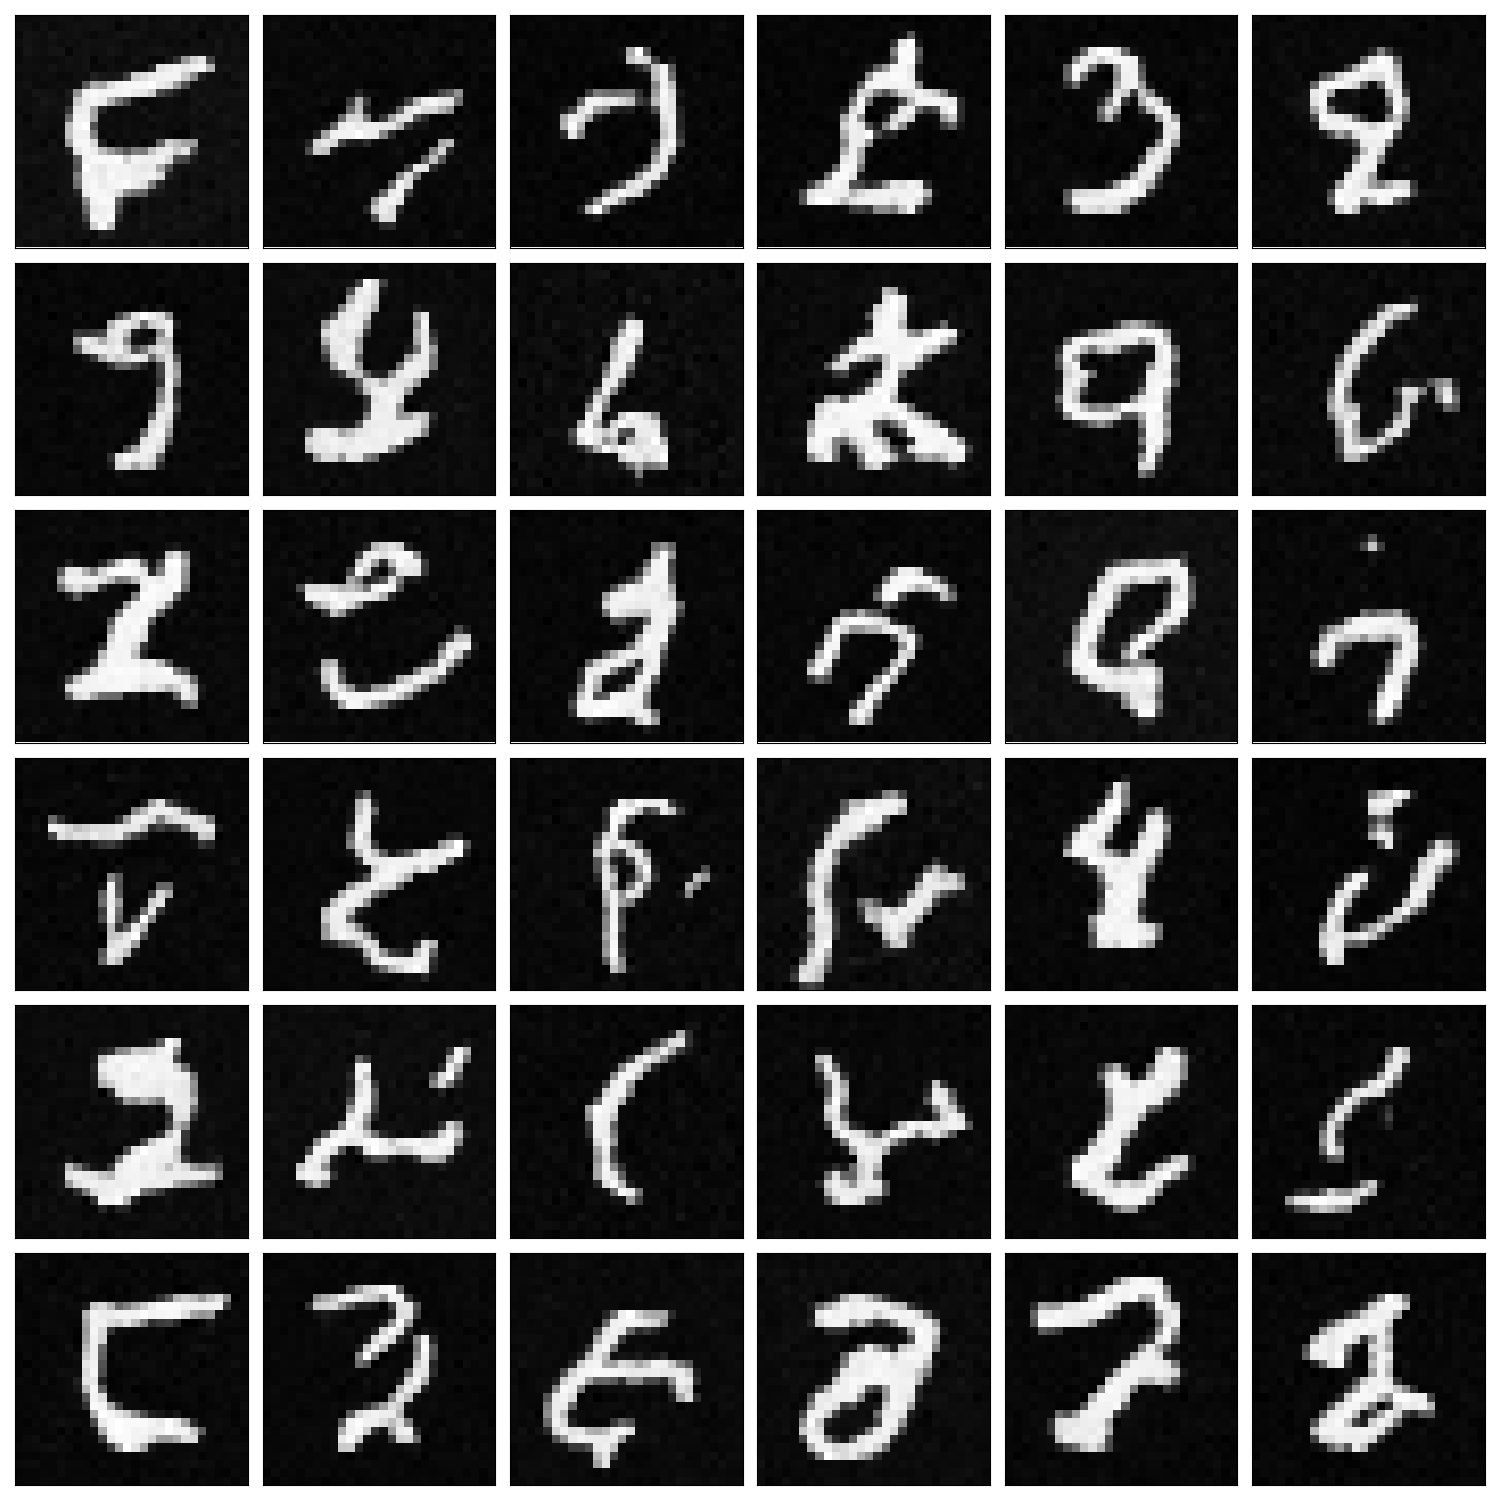
\includegraphics[scale=0.3]{figures/samples_1.png}
    \caption{Samples from model 1.}
    \label{fig:samples_1}
\end{figure}

\begin{figure}[hp]
    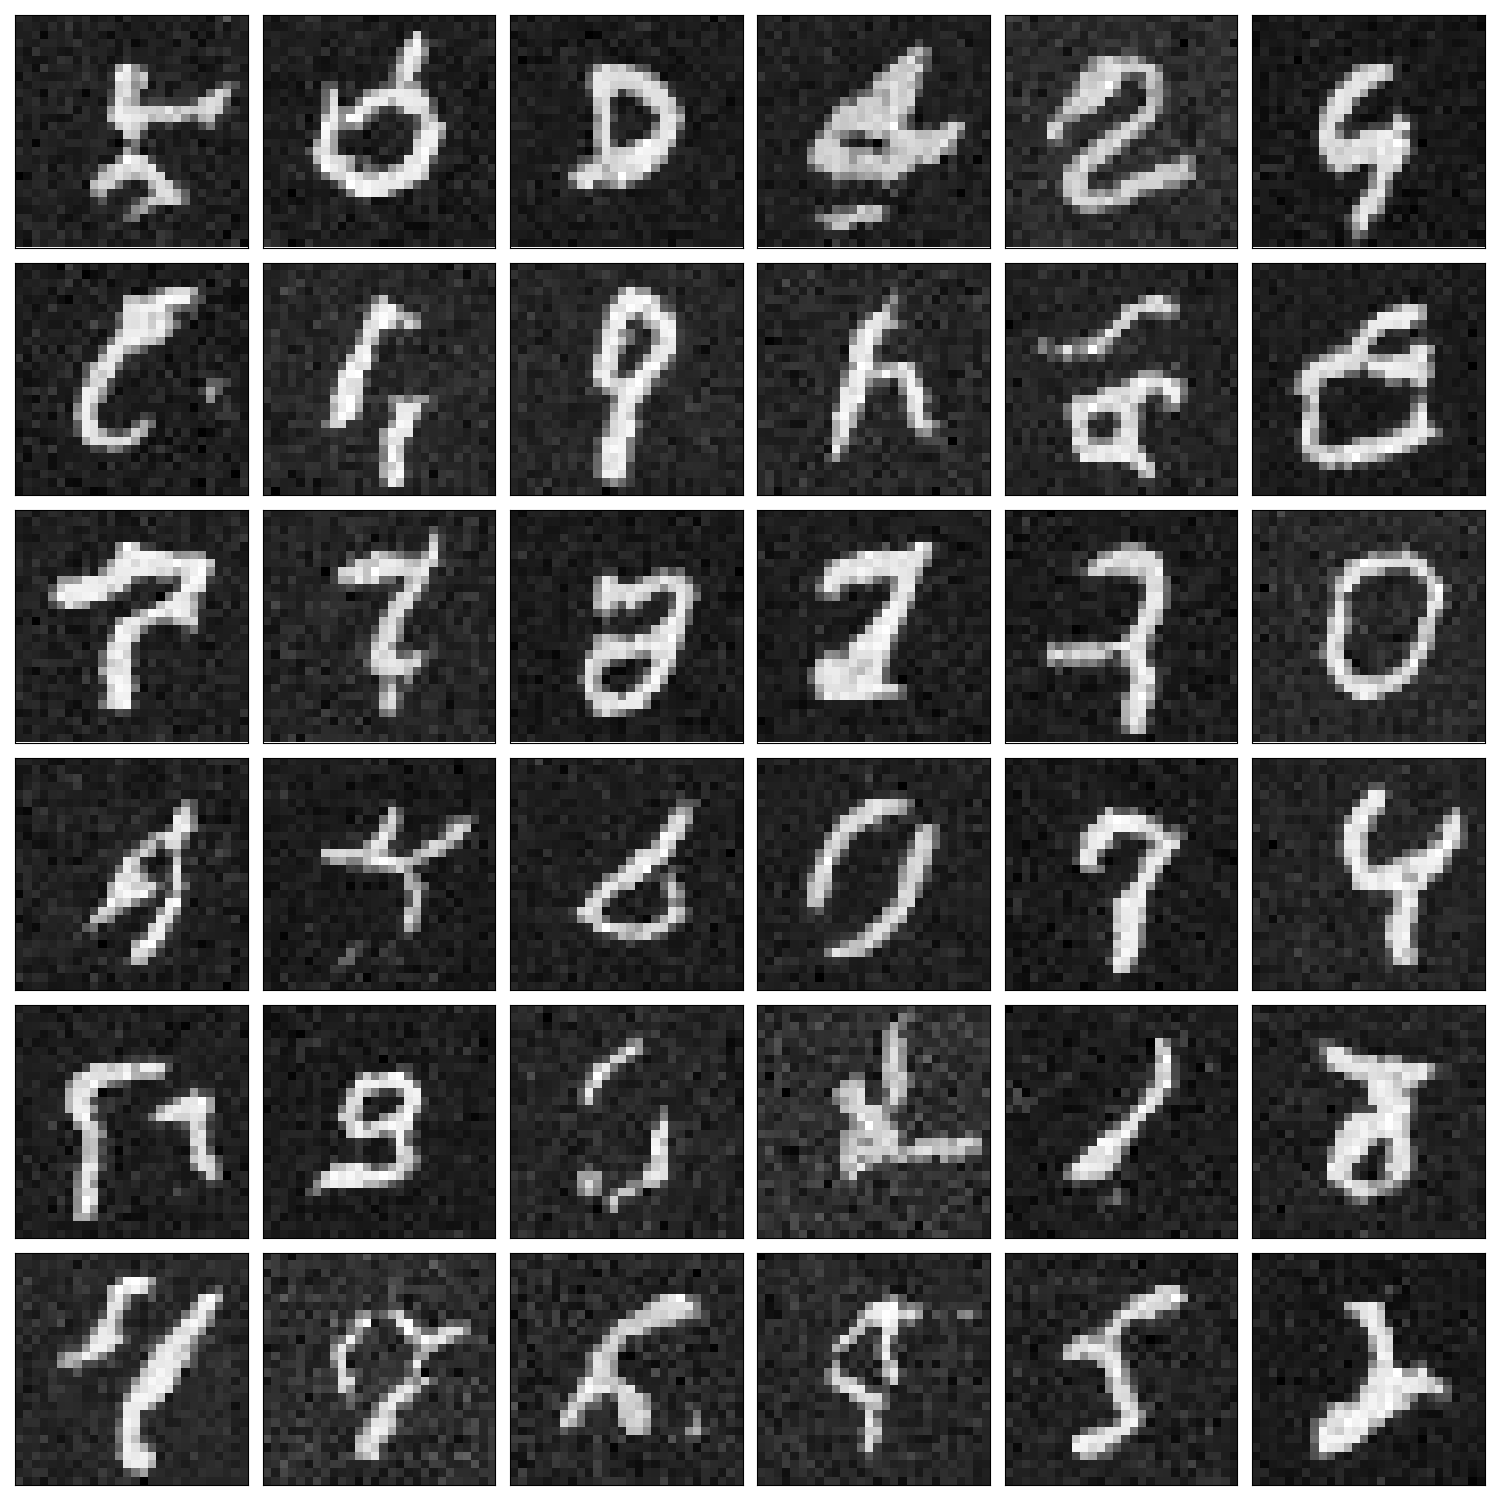
\includegraphics[scale=0.3]{figures/samples_2.png}
    \caption{Samples from model 2.}
    \label{fig:samples_2}
\end{figure}


\section{Custom Diffusion Model}


\subsection{Custom Degradation Strategy}

Earlier prototypes that were infeasible.

Demo plot for digits 1 to 4.
Batch/timestep limitation.


\subsection{Analysis of Custom Degradation Training}
Early epochs diversity issues.
\subsection{Comparison of Gaussian and Custom Degradation}
TSNE plot and Bansal's

\bibliography{Biblio}

\appendix

\section{Statement on the use of auto-generation tools}

Auto-generation tools, such as GitHub or Microsoft Copilot, were not used at any stage during the development of the code within the repository of this project.
Similarly, none of the content of this report was produced -- or proofread -- by modern Large Language Models such as ChatGPT at any point.

\section {High-Performance Computing Resources}

This work was performed using resources provided by the Cambridge Service for Data Driven Discovery (CSD3) operated by the University of Cambridge Research Computing Service (www.csd3.cam.ac.uk),
provided by Dell EMC and Intel using Tier-2 funding from the Engineering and Physical Sciences Research Council (capital grant EP/T022159/1),
and DiRAC funding from the Science and Technology Facilities Council (www.dirac.ac.uk).

\end{document}
